\documentclass{exam}
\printanswers
\usepackage{times}
\usepackage[T1]{fontenc}
\usepackage[portuges]{babel}


% Comentar para not MAC Users
\usepackage[utf8]{inputenc}

\usepackage{a4}
%\usepackage[margin=3cm,nohead]{geometry}
\usepackage{epstopdf}
\usepackage{graphicx}
\usepackage{fancyvrb}
\usepackage{amsmath}
\usepackage{float}
%\renewcommand{\baselinestretch}{1.5}



\begin{document}
\title{Camada de Ligação Lógica: Ethernet e Protocolo ARP}

\author{Etienne Costa(A76089) \and Joana Cruz(A76270) \and Rafael Alves(A72629)}

\date{}
\maketitle

\begin{abstract}
O objectivo deste trabalho é estudar, de uma forma genérica,a camada de ligação lógica. focando
o uso da tecnologia Ethernet e o protocolo ARP.
\end{abstract}
\section{Captura e análise de Tramas Ethernet}

\begin{questions}

\question Anote os endereços MAC de origem e de destino da trama capturada.
\begin{solution}
\begin{figure}[H]
\centering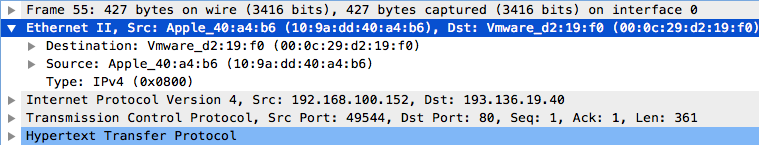
\includegraphics[scale=0.40]{origemdestino} 
\caption{\label{fig:controller}Endereços de origem e destino.}
\end{figure} 
\end{solution}

\question Identifique a que sistemas se referem.Justifique.
\begin{solution}
Source (10:9a:dd:40:a4:b6) : Corresponde ao endereço físico da nossa máquina nativa.
Destination (00:0c:29:d2:19:f0) : Corresponde ao servidor aonde está alocado o site: http://miei.di.uminho.pt.
 \end{solution}

\question Qual o valor hexadecimal do campo Type da trama Ethernet? O que significa?
\begin{solution}
 \begin{equation}
Type= Ox0800. 
\end{equation}
Significa que está a ser transportado num datagrama Ip, que por sua vez está encapsulado no campo de dados de uma trama ethernet.
\end{solution}

\question Quantos bytes são usados desde o início da trama até ao caractere ASCII "G" do método HTTP GET?
Calcule e indique, em percentagem, a sobrecarga (overhead) introduzida pela pilha protocolar no envio do HTTP GET.
\begin{solution}
Até ao caractere "G" temos 66 bytes.
 \begin{equation}
Overhead= \frac{66}{427} = 15,46.
\end{equation}
\end{solution}

\question Através de visualização direta de uma trama capturada, verifique que, possivelmente, o campo FCS(Frame Check Sequence) usado para detecção de erros não está a ser usado. Em sua opinião,porque será?
\begin{solution}
\begin{description}
	\item[•] As redes com vários nós foram substituídas por redes com switches, que geralmente não encaminham pacotes com checksums errados. 
	\item[•] O hardware Ethernet tornou-se muito mais integrado e confiável, tornando-se mais raro precisar de soluções para problemas de baixo nível.  
	\item[•] As codificações da camada física tornaram-se mais complexas, tornando a NIC uma ferramenta menos útil para solucionar problemas nesse nível.
\end{description}
\end{solution}

\question Qual é o endereço Ethernet da fonte? A que sistema de rede corresponde? Justifique.
\begin{solution}
O endereço ethernet da fonte é :
 \begin{equation}
Source:00:0c:29:d2:19:f0
\end{equation}
Corresponde ao servidor aonde está alocado o site: http://miei.di.uminho.pt.
\begin{figure}[H]
\centering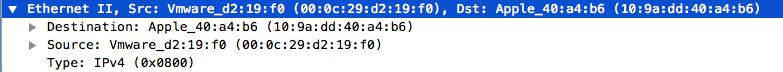
\includegraphics[scale=0.40]{FirstReply} 
\caption{\label{fig:controller}Reply.}
\end{figure} 
\end{solution}
\question Qual é o endereço MAC do destino? A que sistema corresponde?
\begin{solution}
O endereço ethernet do destino é :
 \begin{equation}
Destination: 10:9a:dd:40:a4:b6 
\end{equation}
Corresponde ao endereço físico da nossa máquina nativa.
\end{solution}

\question Atendendo ao conceito de desencapsulamento protocolar, identifique os vários protocolos contidos na trama recebida.
\begin{solution}
Os protocolos contidos na trama recebida são:
\begin{description}
	\item[•] \textbf{Ethernet}.
	\item[•] \textbf{Internet Protocol}. 
	\item[•] \textbf{Transmission Control Protocol}.
	\item[•] \textbf{Hypertext Transfer Protocol}.
\end{description}	
\end{solution}

\section{Protocolo ARP}



\question  Observe o conteúdo da tabela ARP. Diga o que significada cada uma das colunas.
\begin{solution}
Tirando partido do comando arp -a obtemos o seguinte:
\begin{description}
	\item[•] \textbf{Primeira Coluna:} Corresponde aos endereços Ip.
	\item[•] \textbf{Segunda Coluna:} Corresponde aos endereços físicos associados ao IP da primeira coluna. 
	\item[•] \textbf{Quinta Coluna:} Corresponde a interface que estamos a usar que neste caso é ethernet.
\end{description}
\begin{figure}[H]
\centering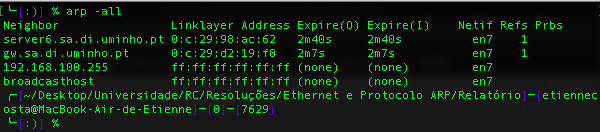
\includegraphics[scale=0.50]{TabelaArp} 
\caption{\label{fig:controller}Arp -all}
\end{figure} 
\end{solution}

\question Qual é o valor hexadecimal dos endereços origem e destino na trama Ethernet que contém a mensagem
com o pedido ARP (ARP Request)? Como interpreta e justifica o endereço destino usado?
\begin{solution}
O endereço destino é o broadcast visto que inicialmente ele não sabe o endereço MAC associado ao IP 192.168.100.227, sendo assim manda para todos que estão ligados
a rede de modo a obter o endereço MAC do 192.168.100.227.
\end{solution}
\begin{figure}[H]
\centering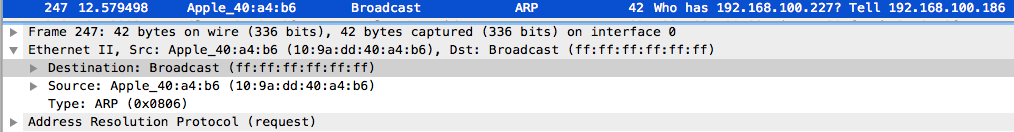
\includegraphics[scale=0.35]{10} 
\caption{\label{fig:controller}Arp Request}
\end{figure} 

\question Qual o valor hexadecimal do campo tipo da trama Ethernet? O que indica?
\begin{solution}
\begin{equation}
Type= Ox0806.
\end{equation}
Indica que o protocolo utilizado na trama em questão é o ARP.
\end{solution}

\question Qual o valor do campo ARP opcode? O que especifica? 
\begin{solution}
 \begin{equation}
Opcode= request (1).
\end{equation}
O opcode indica que tipo de pacote ARP é. Sendo que existem apenas dois valores possíveis para esse opcode, quando o mesmo é igual a 1 indica que é um Request.
\end{solution}

\question Identifique que tipo de endereços estão contidos na mensagem ARP? Que conclui?
\begin{solution}
Na mensagem ARP encontramos dois tipos de endereços que são:
\begin{description}
	\item[•] \textbf{IP:}
	\begin{description}
		\item[•] \textbf{Sender IP Adress:}192.168.100.186
		\item[•] \textbf{Target IP Adress:}192.168.100.227
	\end{description}	
	\item[•] \textbf{MAC:} 
	\begin{description}
		\item[•] \textbf{Sender MAC Adress:}10:9a:dd:40:a4:b6
		\item[•] \textbf{Target MAC Adress:}:00:00:00:00:00:00
	\end{description}	
\end{description}
Sendo que o ARP faz o mapeamento do endereço IP para o endereço MAC podemos, concluir que o Sender MAC Adress e o Target MAC Adress são resultados desse mapeamento dos respectivos valores do Sender IP Adress e Target IP Adress, embora o Target MAC Adress ainda seja tudo a zeros visto que ainda não se sabe o seu verdadeiro valor.
\end{solution}
\begin{figure}[H]
\centering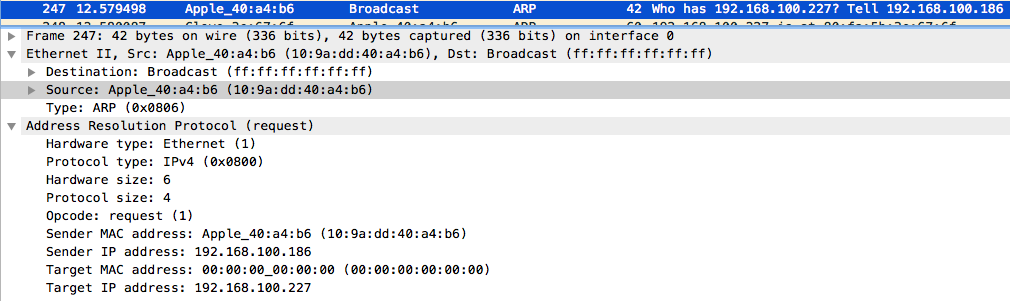
\includegraphics[scale=0.35]{13} 
\caption{\label{fig:controller}Arp Request}
\end{figure}

\question Explicite que tipo de pedido ou pergunta é feita pelo host de origem?
\begin{solution}
"Who has 192.168.100.227? Tell 192.168.100.186"
 O host envia uma pergunta ARP para descobrir qual o endereço MAC cujo endereço IP é  192.168.100.227, sendo que essa pergunta na rede é feita em
 broadcast.
\end{solution}

\question Localize a mensagem ARP que é a resposta ao pedido ARP efectuado.
\begin{figure}[H]
\centering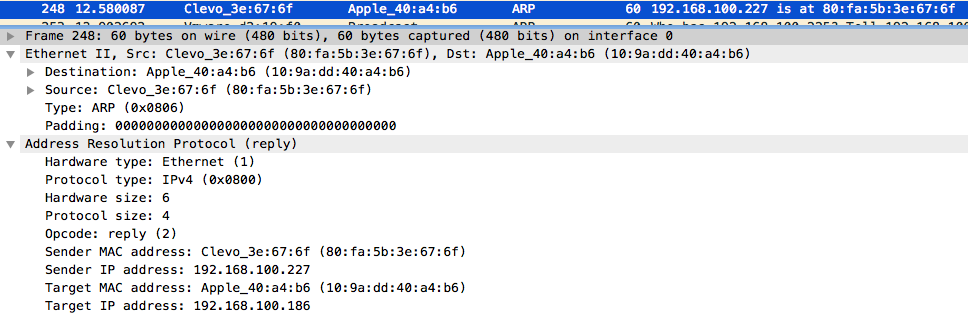
\includegraphics[scale=0.35]{15} 
\caption{\label{fig:controller}Arp Reply}
\end{figure}

\question Qual o valor do campo ARP opcode? O que especifica?
\begin{solution}
 \begin{equation}
Opcode= reply (2).
\end{equation}
O opcode indica que tipo de pacote ARP é. Sendo que existem apenas dois valores possíveis para esse opcode, quando o mesmo é igual a 2 indica que é um Reply.
\end{solution}

\question Em que posição da mensagem ARP está a resposta ao pedido ARP?
\begin{solution}
A resposta ao pedido arp tem início no byte 14 sendo que o Mac Adress do IP em questão se encontra no byte 23.
\begin{figure}[H]
\centering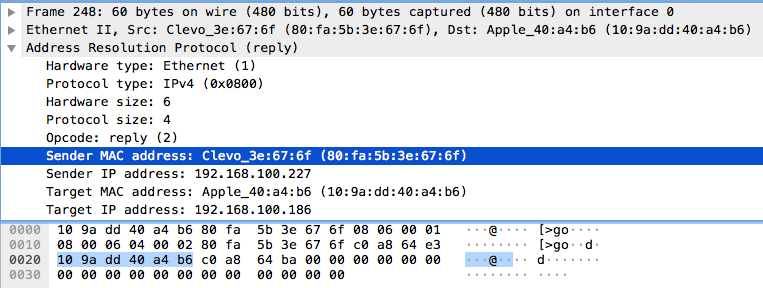
\includegraphics[scale=0.40]{PosicaoArp} 
\caption{\label{fig:controller}Posição da resposta ao pedido Arp.}
\end{figure}
\end{solution}



\section{ARP Gratuito}

\question Identifique um pacote de pedido ARP gratuito originado pelo seu sistema.
Analise o conteúdo de um pedido ARP gratuito e identifique em que se distingue dos restantes pedidos ARP.Registe a trama Ethernet correspondente. Qual o resultado esperado face ao pedido ARP gratuito enviado?
\begin{solution}
A primeira grande diferença que podemos constatar é que existe uma flag [Is gratuitous:True] que indica que se trata de um pedido Arp
gratuito e o arp gratuito distingue-se dos outros pois possuí o mesmo IP no campo Sender IP Adress e Target Ip Adress.
O resultado esperado face ao pedido Arp gratuito é não haver mais replies porque , caso houvesse , haveria endereços Ip's duplicados.
Saber se o Ip está ou não a ser utilizado nesta rede.
\end{solution}
\begin{figure}[H]
\centering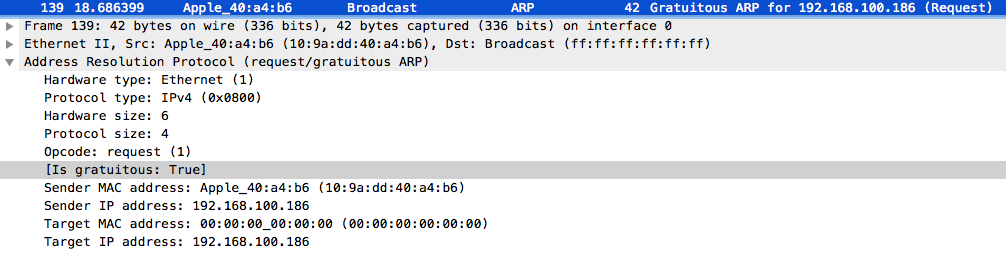
\includegraphics[scale=0.45]{ArpGratuito} 
\caption{\label{fig:controller}Arp Gratuitous.}
\end{figure}

section{Domínios de colisão}

\question Faça ping de n1 para n2. Verifique com a opção tcpdump como flui o tráfego nas diversas interfaces dos vários dispositivos.Que conclui?

\begin{figure}[H]
\centering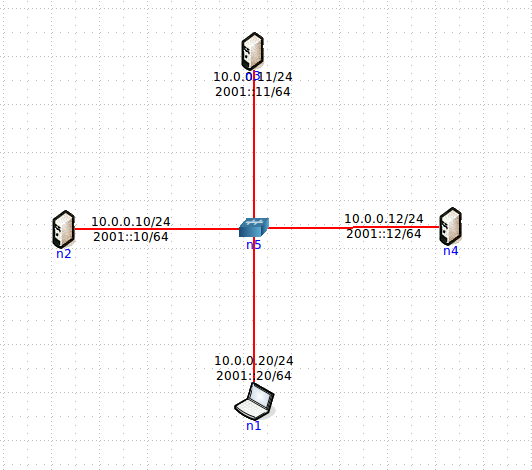
\includegraphics[scale=0.45]{topologiaHub} 
\caption{\label{fig:controller}Topologia Core Hub.}
\end{figure}
\begin{figure}[H]
\centering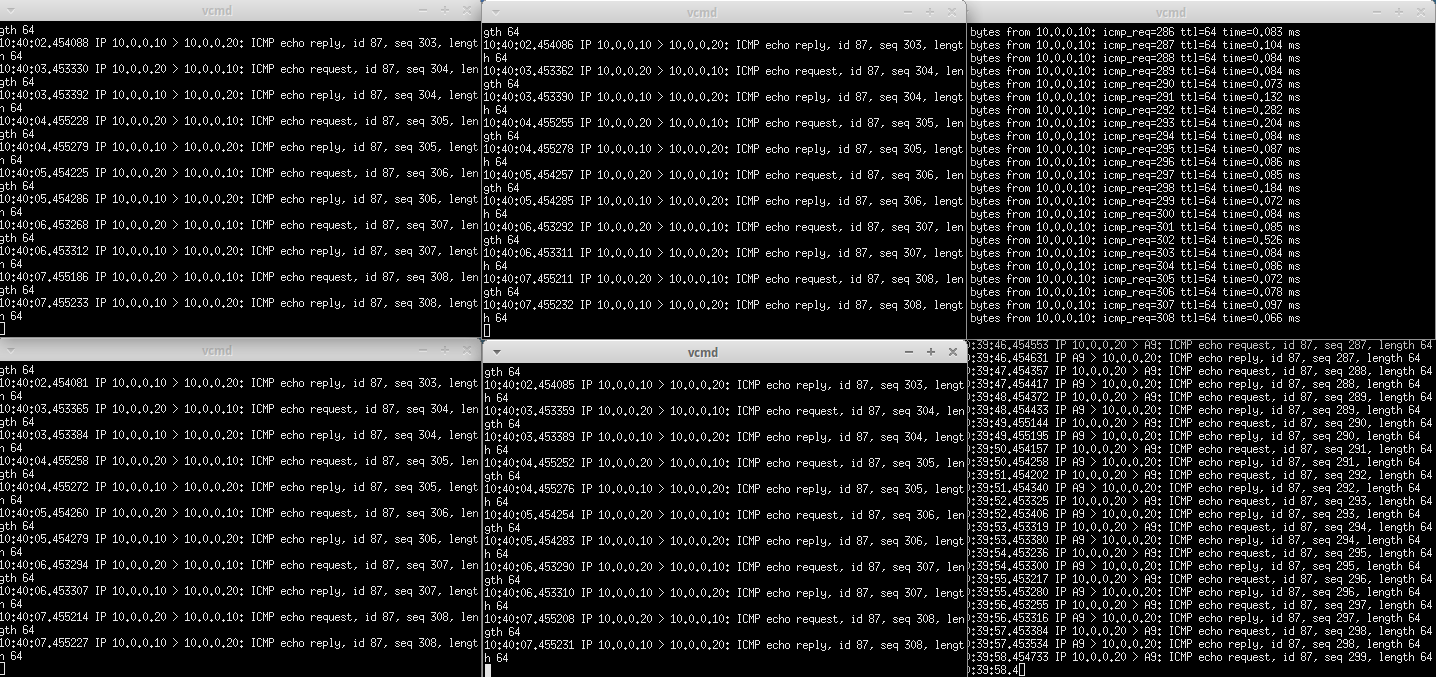
\includegraphics[scale=0.45]{tcpdumpHUB} 
\caption{\label{fig:controller}Trafego com um hub de interligação.}
\end{figure}

\begin{solution}
Visto que o equipamento de interligação se trata um hub(repetidor), este irá encaminhar
os datagramas para todas as suas interfaces de saída e, portanto, o output do tcpdump será o mesmo
em todas as interfaces dos dispositivos ligados ao hub, apesar da troca de mensagens ser entre o host n1 e o host n2. 
\end{solution}

\question Na topologia de rede substitua o hub por um switch. Repita os procedimentos que realizou na pergunta anterior .
Comente os resultados obtidos quantos à utilização de hubs e switches no contexto de controlar ou dividir domínios de colisão. Documente as suas observações e conclusões com base no tráfego observado/capturado.
\begin{figure}[H]
\centering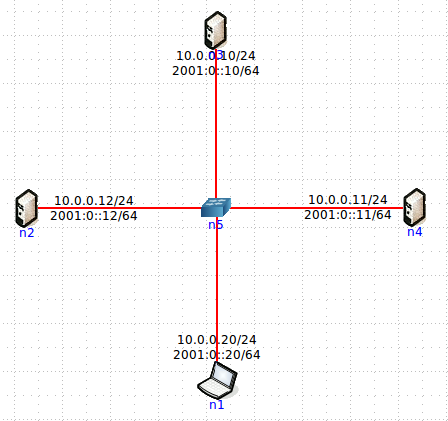
\includegraphics[scale=0.45]{topologiaSwitch} 
\caption{\label{fig:controller}Topologia Core Switch.}
\end{figure}

\begin{figure}[H]
\centering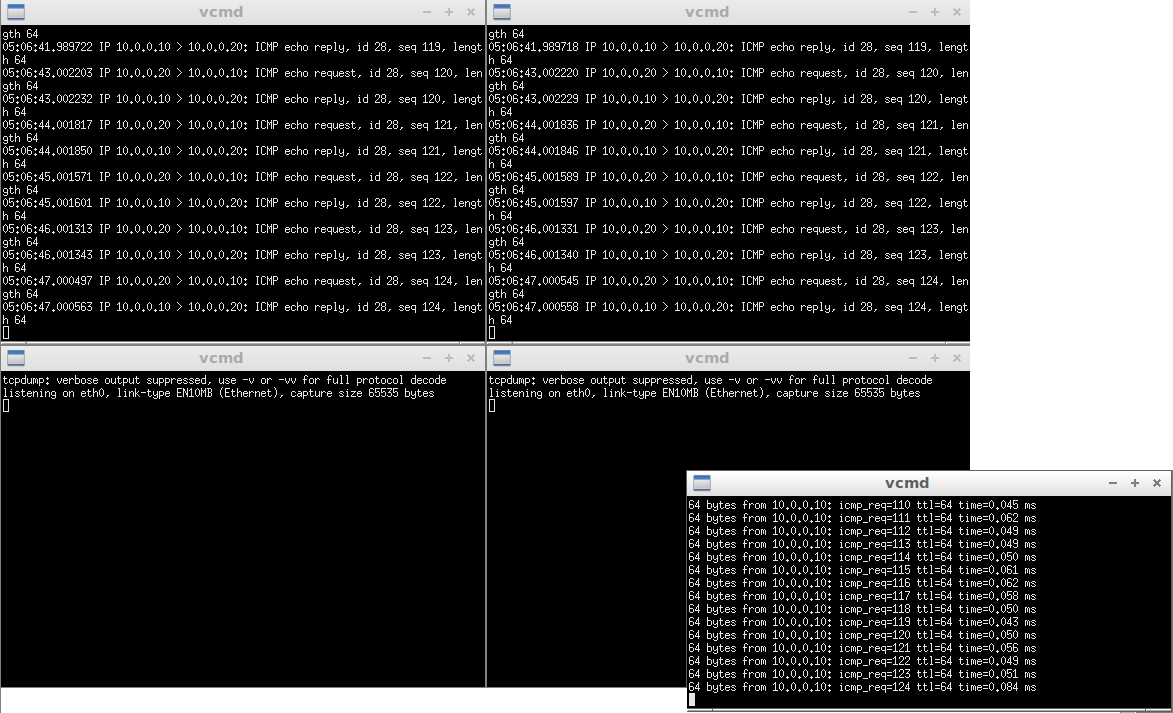
\includegraphics[scale=0.45]{tcpDumpTodosSwitch} 
\caption{\label{fig:controller}Trafego com um switch de interligação.}
\end{figure}

\begin{solution}
Visto agora o equipamento de interligação ser um switch, o encaminhamento é feito para a interface associada ao MAC adress destino de cada 
datagrama, como tal o tcpdump apenas apresentará output nos hosts envolvidos na operação ping, respetivamente os hosts n1 e n2.
\end{solution}

\end{questions}

\section{Conclusão}
O MAC Address tem um papel central na camada de ligação de dados permitindo identificar, de forma unívoca, uma NIC estando na base de protocolos como Ethernet que definem formas de acesso ao meio. Por outro lado, visto tratar-se de um endereço físico, surgiram protocolos como o ARP(Address Resolution Protocol) que mapeiam estes endereços em endereços IP permitindo assim a entrega de dados entre nós adjacentes (i.e. na mesma rede local). Este protocolo (ARP) pode ainda ser usado para deteção de endereços IP repetidos na mesma rede (local), tendo a desginação de ARP Gratuito quando  é usado para este fim. Por fim, a ligação de equipamentos numa rede local implica a ocorrência (ocasional) de colisões derivado do facto de haver um meio partilhado de transmissão de dados entre hosts. A ocorrência de colisões pode ser evitada através do recurso a protocolos de
 acesso ao meio (nomeadamente CSMA/CD implementado pelo protocolo Ethernet) ou através do uso de aparelhos de ligação denominados switches.

\end{document}